\section{Algorithm Description}
\subsection{Genetic Algorithm}
\label{ssec:GenAlg}
The algorithm must determine positions and number of luminaries in dependency on target illuminance and uniformity. This is the multicriteria and multiparametric type of the problem. The genetic algorithm offer quite simple way how to solve it, therefore they were used in this case. The genetic algorithms are well known today so only specific settings are further described.

The best solution was saved (elitism) from every population in two specimens. The first one was unable to change its DNA via mutation, the second one had the same probability of mutation like other solutions. Other parent solutions were selected via tournament selection. It consisted of making random group of $4$ solutions from the population and take the one with the best fitness. This type of selection had vital role for the algorithm. It avoided premature convergence of the best solution in comparison with the roulette selection. Similar effect was ensured also by recombination probability set less than $1$. There was used just one point crossover during the tests. Overview of the all GA settings is shown in table~\ref{tab:GAsettings}.

\begin{table}[htb]
	\renewcommand{\arraystretch}{1.3}
	\caption{Genetic Algorithm Settings}
 	\label{tab:GAsettings}
	\centering
  \begin{tabular}{| c | c |}
    \hline
    \textbf{First Population} & Random logic vectors \\
    \hline
    \textbf{Termination Cond.} & Maximum number of generations \\
    \hline
		\textbf{Number of Gen.} & $60$ \\
    \hline
		\textbf{Population Size} & $50$ \\
    \hline
		\textbf{Recombination Prop.} & $90 \%$ \\
    \hline
		\textbf{Mutation Prop.} & $5 \%$ \\
    \hline
		\textbf{Parent Selec.} & Tournament 1 of 4 \\
    \hline
		\textbf{Mutation Mech.} & Inverted bit \\
    \hline
		\textbf{Survival Selec.} & Elitism \\
    \hline
  \end{tabular}
\end{table}

\subsection{Fitness Function}
\label{ssec:FitFn}
The fitness function defines how good the solutions are. The target value of average illuminance and target value of uniformity are watched in the algorithm. In common case the average illuminance is given especially by number of the lamps. The uniformity is given especially by placement of the lamps on the other hand. The count of the lamps is proportional to the investment cost to the lighting system. So the number of lamps that exactly fulfill the target average value of illuminance is appropriate. The uniformity is always required as much as possible for defined number of lamps. Therefore the fitness function was determined within discussed facts as follows:

\begin{equation}
\label{eq:fitness}
f_{DNA}\left(E_{avg}, U_0\right) = g_1\left(E_{avg}\right) + g_2\left(U_0\right)
\end{equation}

\begin{subnumcases}{\label{eq:fitnessG1} g_1\left(E_{avg}\right)=} 
  e^{\frac{E_{avg}-E_{avgT}}{E_{avg}}} &, $\left\langle 0, E_{avgT}\right\rangle$ \label{eq:fitnessG1A}\\
  e^{\frac{E_{avgT}-E_{avg}}{E_{avg}}} &, $\left( E_{avgT}, \infty\right)$ \label{eq:fitnessG1B}
\end{subnumcases}

\begin{subnumcases}{\label{eq:fitnessG2} g_2\left(U_0\right)=} 
  \frac{U_0}{2\cdot U_{0T}} &, $\left\langle 0, U_{0T}\right\rangle$ \label{eq:fitnessG2A}\\
  1-\frac{e^{U_{0T}-U_0}}{2} &, $\left( U_{0T}, \infty\right)$ \label{eq:fitnessG2B}
\end{subnumcases}

where:
\begin{description}
	\item[$E_{avg}$] is a calculated average value of illuminance,
	\item[$E_{avgT}$] is a target average value of illuminance,
	\item[$U_0$] is a calculated uniformity,
	\item[$U_{0T}$] is a target uniformity.
\end{description}

The function $g_1\left(E_{avg}\right)$ has peak value equal to $1$ at target value of average illuminance. Because the illuminance cannot be less than zero, the function reaches two limits:
\begin{equation}
\label{eq:g1lim0}
\lim_{E_{avg}\to 0+} g_1\left(E_{avg}\right) = 0
\end{equation}
\begin{equation}
\label{eq:g1limInf}
\lim_{E_{avg}\to \infty} g_1\left(E_{avg}\right) = e^{-1}
\end{equation}

Both limits have different values and the limit in infinity is higher than that in the $0$. This means that for the same absolute difference from the target value is preferred the solution with the higher average illuminance.

\begin{figure}[htb]
  \centering
  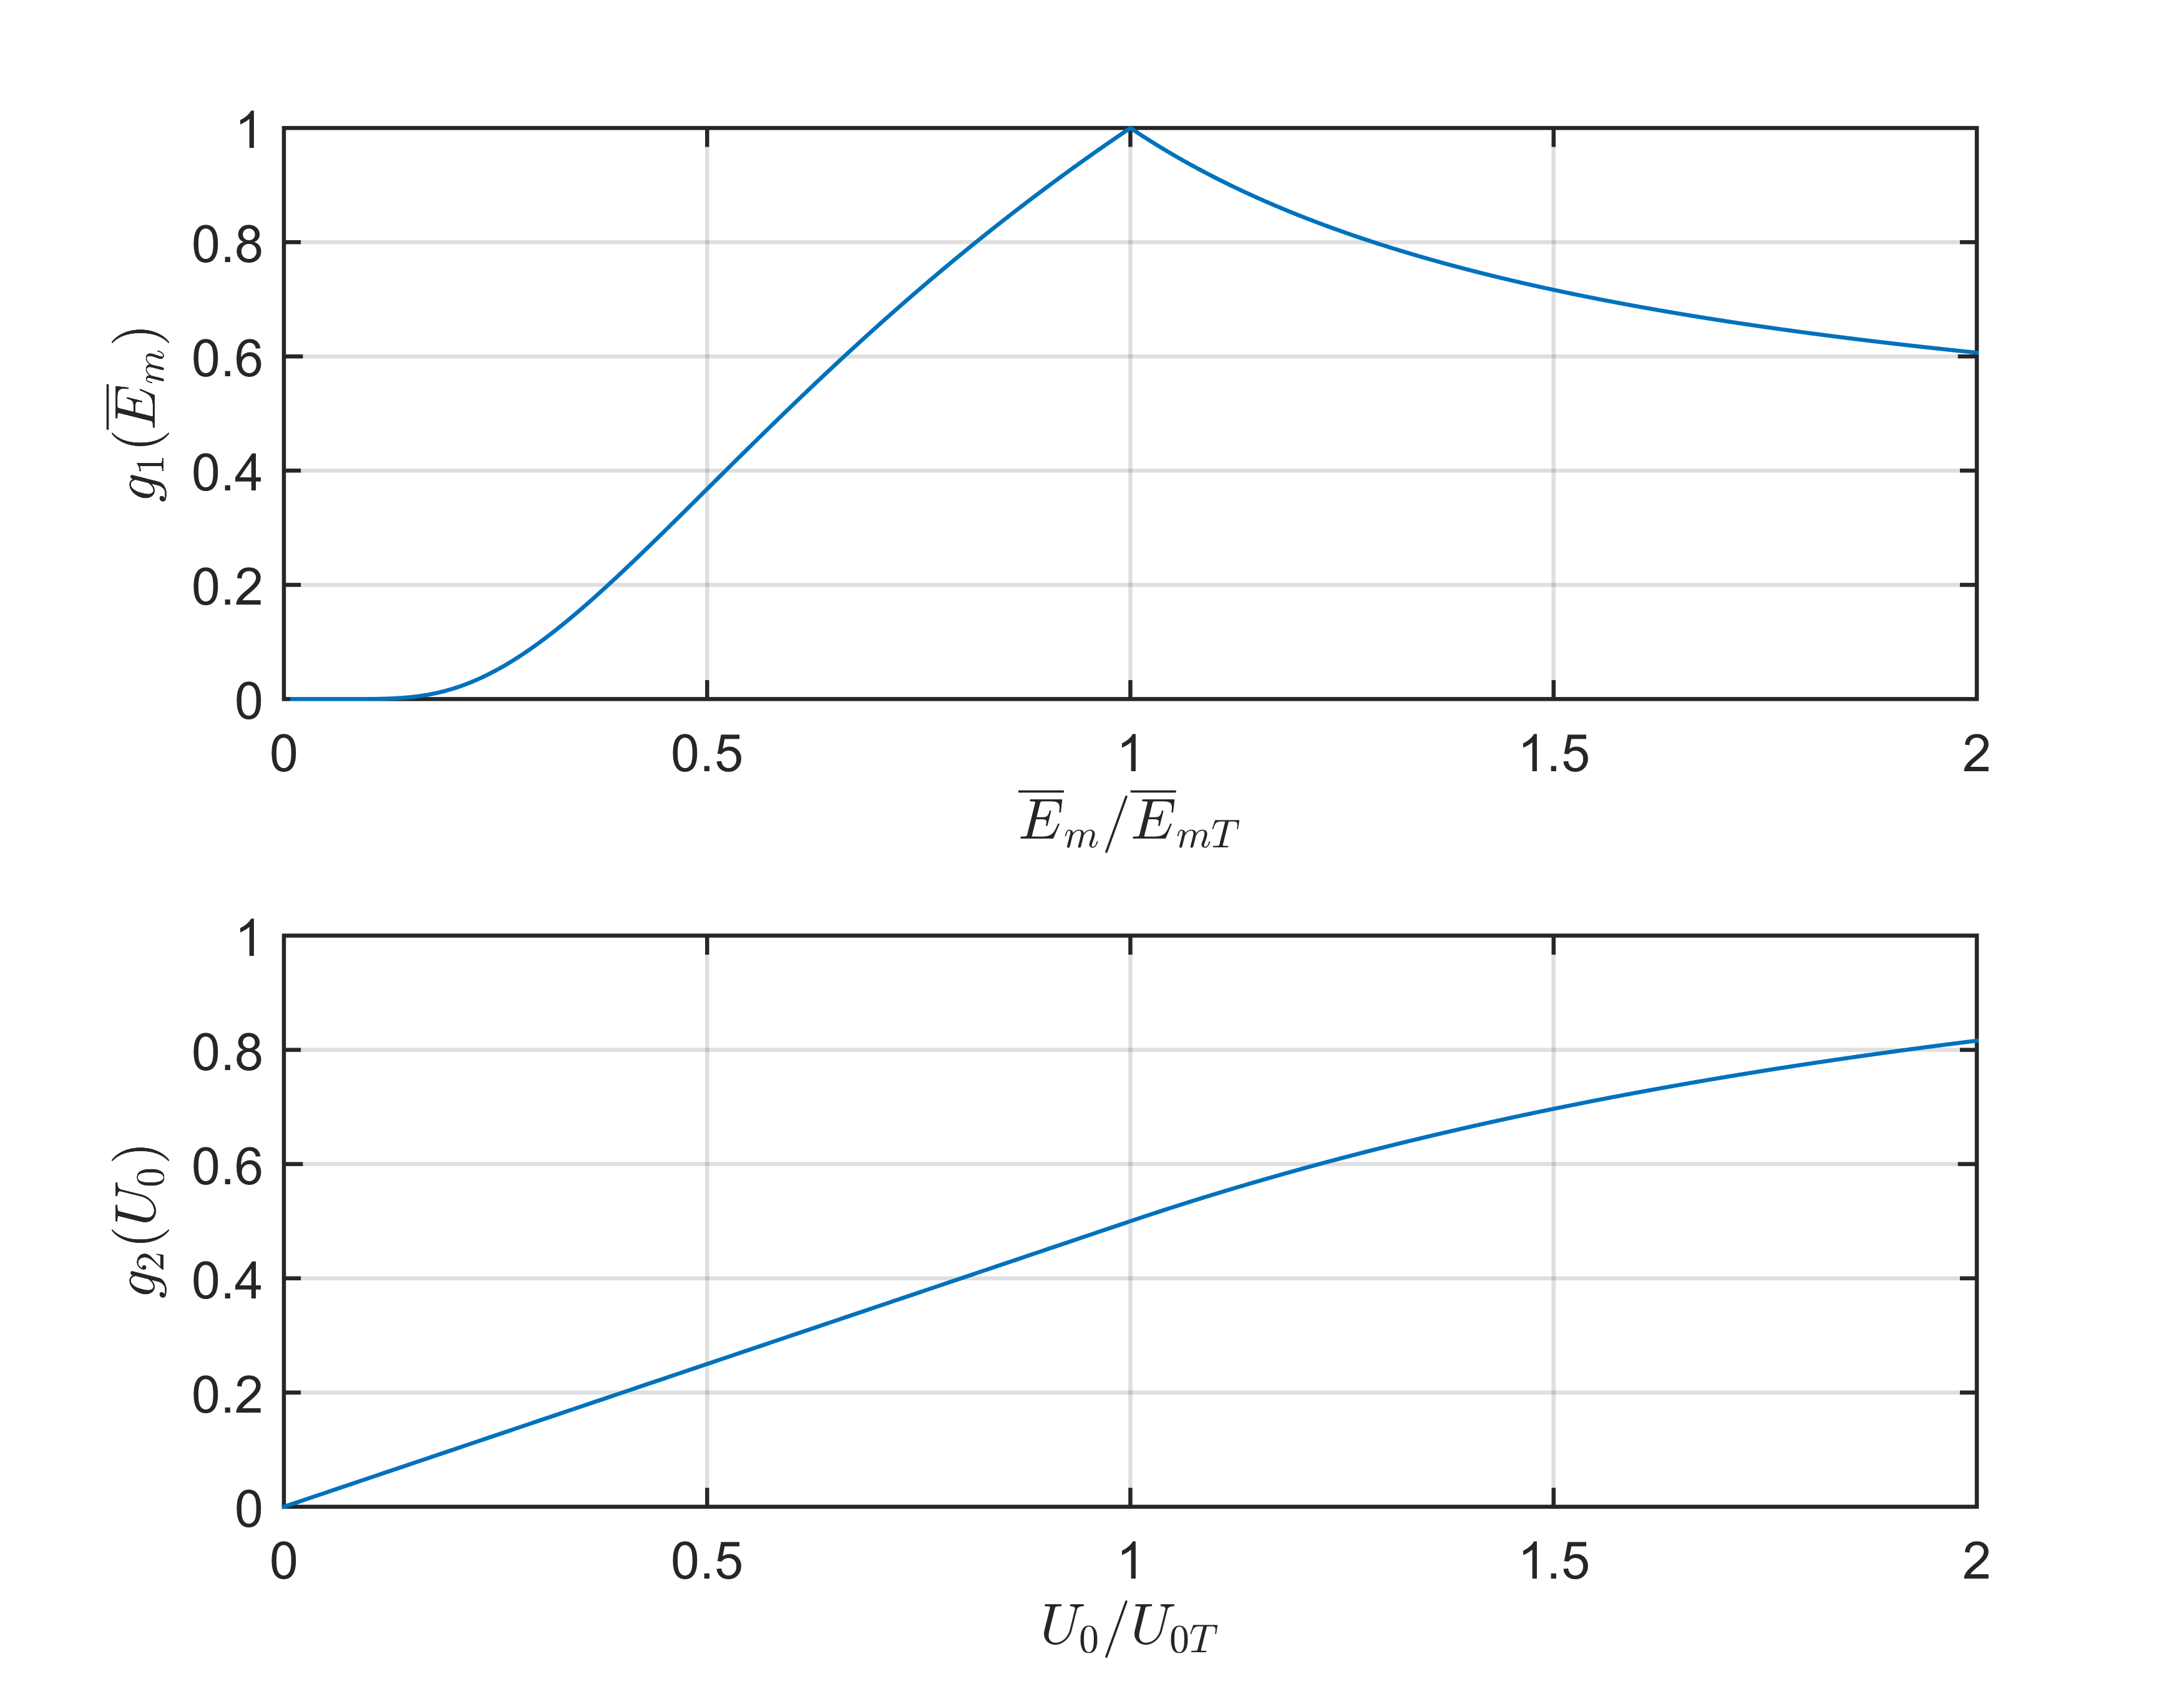
\includegraphics[width=\columnwidth]{obrG1G2}
  \caption{Graphs of parts $g_1\left(E_{avg}\right)$ and $g_2\left(U_0\right)$ from the fitness function}
  \label{fig:sidewalk}
\end{figure}

The function $g_2\left(U_{0}\right)$ reach value $0.5$ at target value of uniformity. It has a bound at $0$ for values less then target value. There is a limit for values in interval higher than target value:
\begin{equation}
\label{eq:g2limInf}
\lim_{U_{0}\to \infty} g_2\left(U_{0}\right) = 1
\end{equation}